\chapter{Batch Service}
\section{Abstract}
The batch micro-service is a major component of this micro-service system. It communicates with the user micro-service which gives individual details about each user in the system. They are tied together with keys but stored individually in completely different databases. The batch micro-service stores batch data within the batch repository. From here, it can send data to any other micro-service that needs batch data.

\section{Batch Architecture}

\begin{figure}[htp]
\centering
\includegraphics[width=18cm]{images/batch-package}
\includegraphics[width=18cm]{images/batch-class}
\caption{Batch Service Infrastructure}
\label{fig:lion}
\end{figure}


\begin{figure}[htp]
\centering
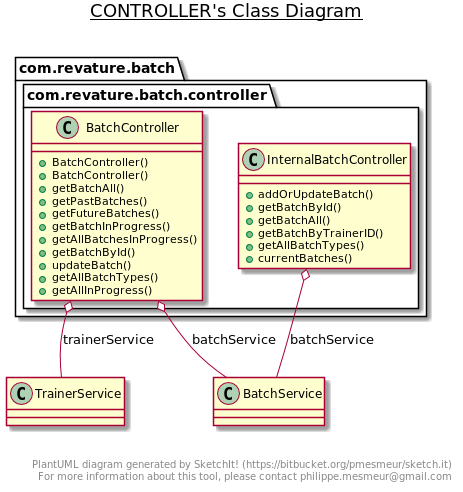
\includegraphics[width=5cm]{images/Batchcontroller}
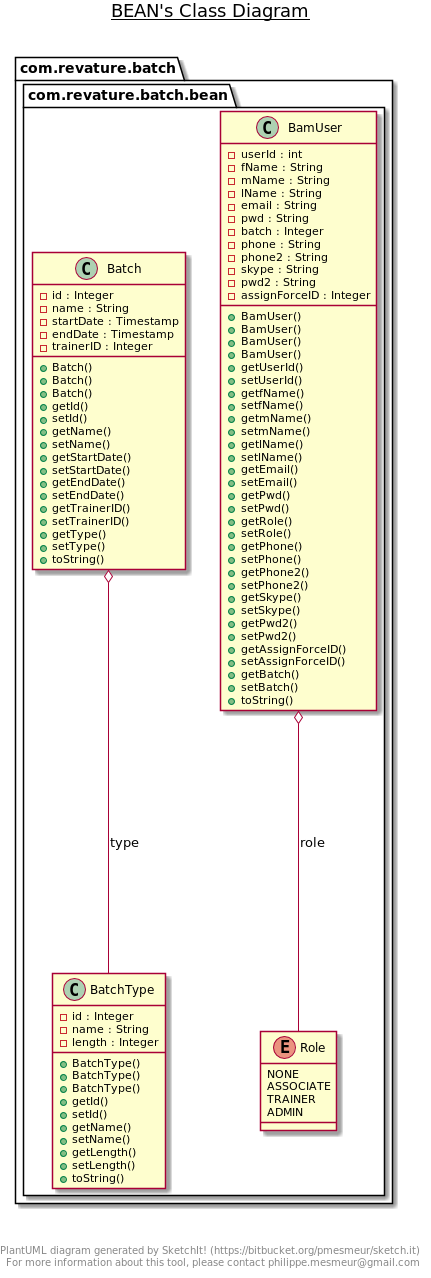
\includegraphics[width=5cm]{images/Batchbean}
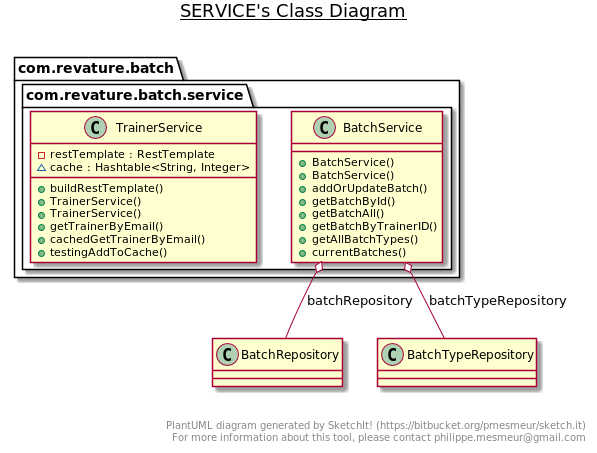
\includegraphics[width=5cm]{images/Batchservice}
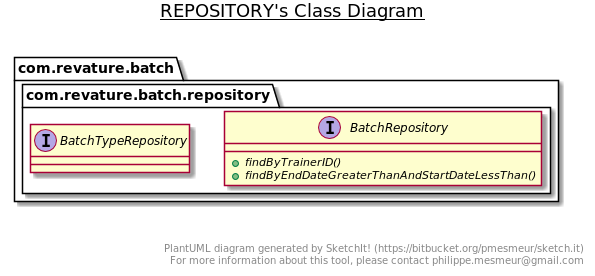
\includegraphics[width=5cm]{images/Batchrepository}
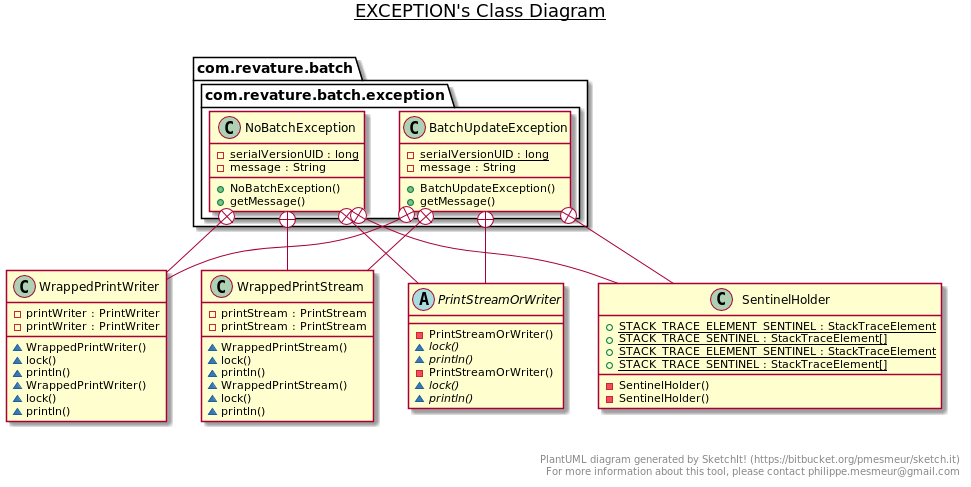
\includegraphics[width=5cm]{images/Batchexception}
\caption{Batch Service Hierarchy}
\label{fig:lion}
\end{figure}